\documentclass{article}
\usepackage[utf8]{inputenc} %кодировка
\usepackage[T2A]{fontenc}
\usepackage[english,russian]{babel} %русификатор 
\usepackage{mathtools} %библиотека матеши
\usepackage[left=1cm,right=1cm,top=2cm,bottom=2cm,bindingoffset=0cm]{geometry} %изменение отступов на листе
\usepackage{amsmath}
\usepackage{graphicx} %библиотека для графики и картинок
\graphicspath{}
\DeclareGraphicsExtensions{.pdf,.png,.jpg}
\usepackage{subcaption}
\usepackage{pgfplots}
\usepackage{float}

\begin{document}
% НАЧАЛО ТИТУЛЬНОГО ЛИСТА
\begin{center}
    \Large
    Федеральное государственное автономное \\
    образовательное учреждение высшего образования \\ 
    «Научно-образовательная корпорация ИТМО»\\
    \vspace{0.5cm}
    \large
    Факультет программной инженерии и компьютерной техники \\
    Направление подготовки 09.03.04 Программная инженерия \\
    \vspace{1cm}
    \Large
    \textbf{Отчёт по лабораторной работе №2} \\
        По дисциплине «Компьютерные сети» ( семестр 6)\\
    \large
    \vspace{8cm}

    \begin{minipage}{.33\textwidth}
    \end{minipage}
    \hfill
    \begin{minipage}{.4\textwidth}
    
        \textbf{Студент}: \vspace{.1cm} \\
        \ Дениченко Александр P3312\\
        \textbf{Практик}:  \\
        \ Тропченко Андрей Александрович
    \end{minipage}
    \vfill
Санкт-Петербург\\ 2025 г.
\end{center}
\pagestyle{empty}
% КОНЕЦ ТИТУЛЬНОГО ЛИСТА 
\newpage
\pagestyle{plain}

\section*{Цель работы}
Изучение принципов настройки и функционирования локальных сетей,
построенных с использованием концентраторов и коммутаторов, а также
процессов передачи данных на основе стека протоколов TCP/IP, с
использованием программы моделирования компьютерных сетей NetEmul.
\begin{itemize}
    \item построить три модели локальной сети: с использованием концентратора,
    коммутатора и многосегментную сеть;
    \item выполнить настройку сети, заключающуюся в присвоении IP-адресов
    интерфейсам сети;
    \item выполнить тестирование разработанных сетей путем проведения
    экспериментов по передаче данных (пакетов и кадров) на основе
    протоколов UDP и TCP;
    \item проанализировать результаты тестирования и сформулировать выводы об
    эффективности смоделированных вариантов построения локальных сетей;
    \item сохранить разработанные модели локальных сетей для демонстрации
    процессов передачи данных при защите лабораторной работы.
\end{itemize}

\section*{Вариант}

Ф=9; И=9; О=8; Н=12
\\ 
сети 1 = 2
\\
сети 2 = 4
\\
сети 3 = 3
\\
Класс IP-адресов = В
\\
для класса В:
(И+Н+128).(О+Н).(Ф+Н).(Ф+И) = (9+12+128).(8+12).(9+12).(9+9) = 149.20.21.18 (диапазон от 128 до 191)

\section{Построение сети с концентратором}

Для построения сети пронумеруем интерфейсы компьютеров: 149.20.21.18 и 149.20.21.19

\begin{center}
    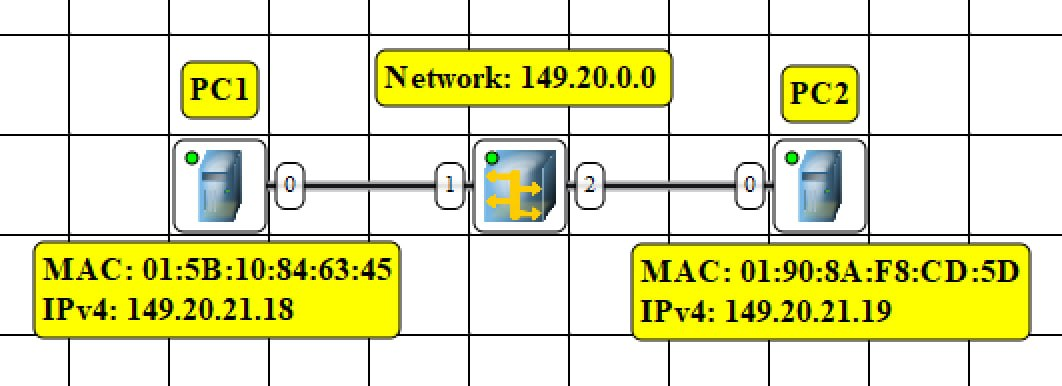
\includegraphics[width=.9\textwidth]{con-1.jpg}
\end{center}

После соединения с концентратором компьютеры обменялись своими MAC адресами через ARP реквесты.
\\
Таблицы маршрутизации выглядят следующим образом.

\begin{minipage}{.5\textwidth}
    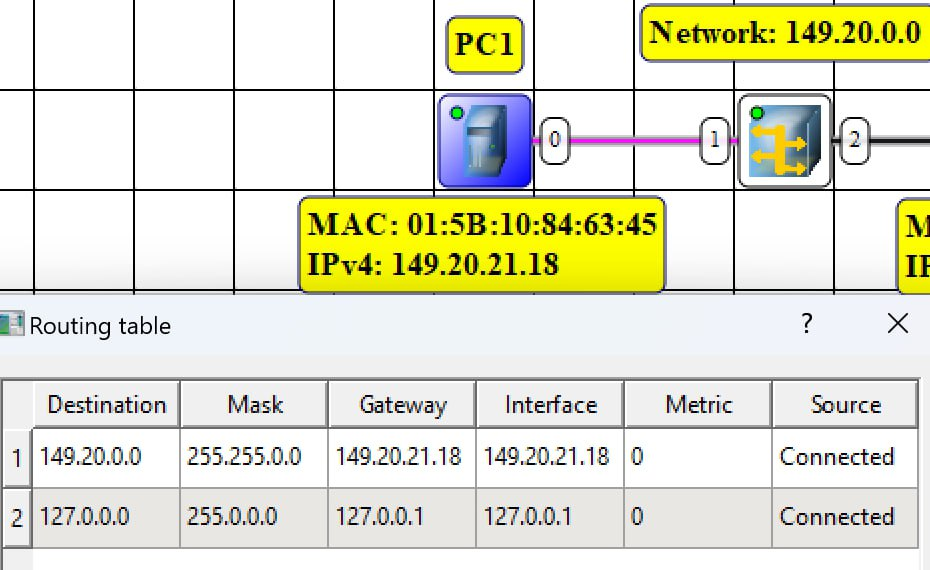
\includegraphics[width=.9\textwidth]{conc-2.jpg}
\end{minipage}
\hfill
\begin{minipage}{.5\textwidth}
    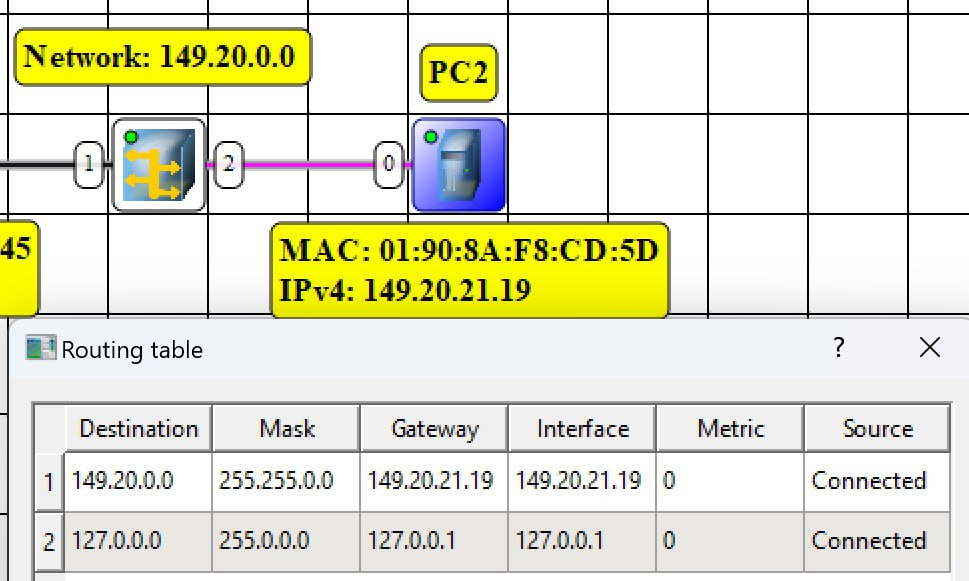
\includegraphics[width=.9\textwidth]{conc-3.jpg}
\end{minipage}

ARP таблицы заполнились у компьютеров только после arp реквестов, там отобразились динамически MAC адреса, у которыйх есть некоторый time limit.
\\
\begin{center}
    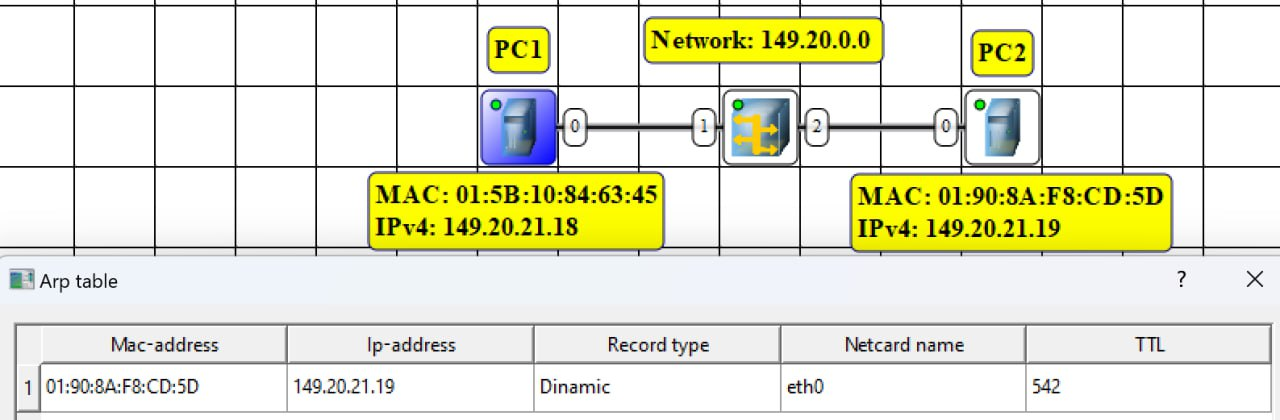
\includegraphics[width=.9\textwidth]{conc-6.jpg}
\end{center}
\begin{center}
    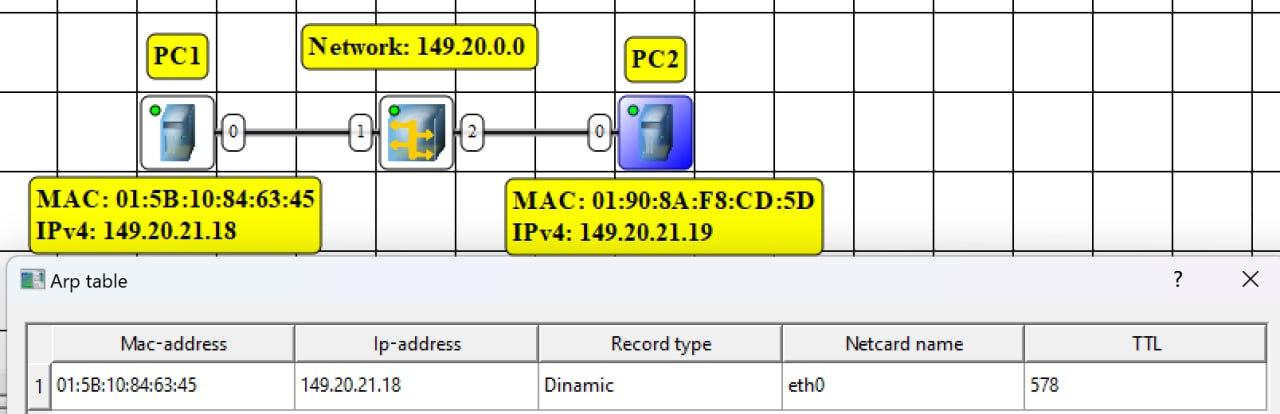
\includegraphics[width=.9\textwidth]{conc-7.jpg}
\end{center}
Для проверки работы сети, была проведена отправка данных по UDP.

\begin{center}
    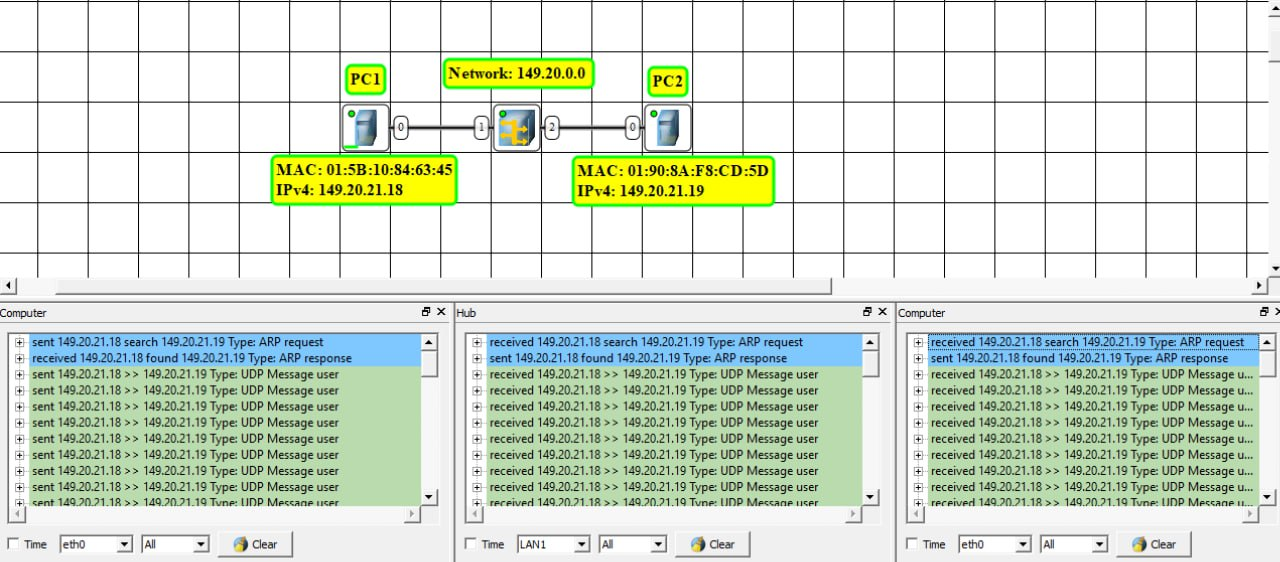
\includegraphics[width=.9\textwidth]{conc-4.jpg}
\end{center}
Подробное содержание сообщений. Сначала идёт отправка пакета с кадром ARP - запроса. Если приходит ответ, то тогда отправляется Ethernet пакет с IP пакетом, а так же сегмент данных по UDP.


\begin{center}
    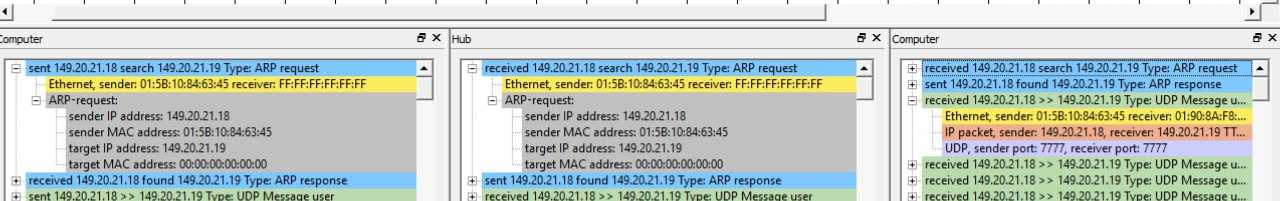
\includegraphics[width=.9\textwidth]{conc-5.jpg}
\end{center}

Ещё было протестировано TCP/IP соединение

\begin{center}
    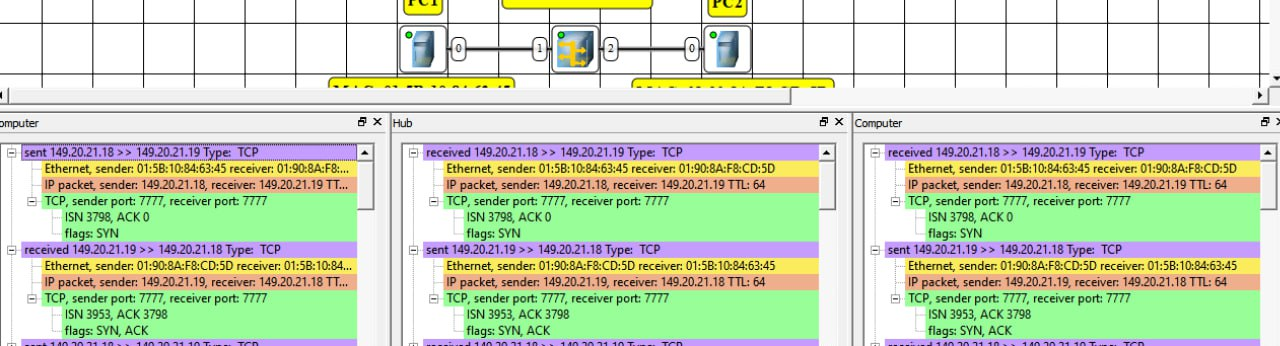
\includegraphics[width=.9\textwidth]{conc-8.jpg}
\end{center}

\section{Локальная сеть с коммутатором}
В сети не пришлось ничего настраивать вручную, так как по умолчанию портов в коммутаторе 4 штуки.
При подключении компьютеров к коммутатору, всем от этого компьютера рассылается ARP запрос, чтобы показать, что в сети появился новый компьютер, при этом записи в таблицах динамические (300 сек).
В самом коммутаторе тоже вписываются динамически занятые порты при пересылке ARP запросов.
\begin{center}
    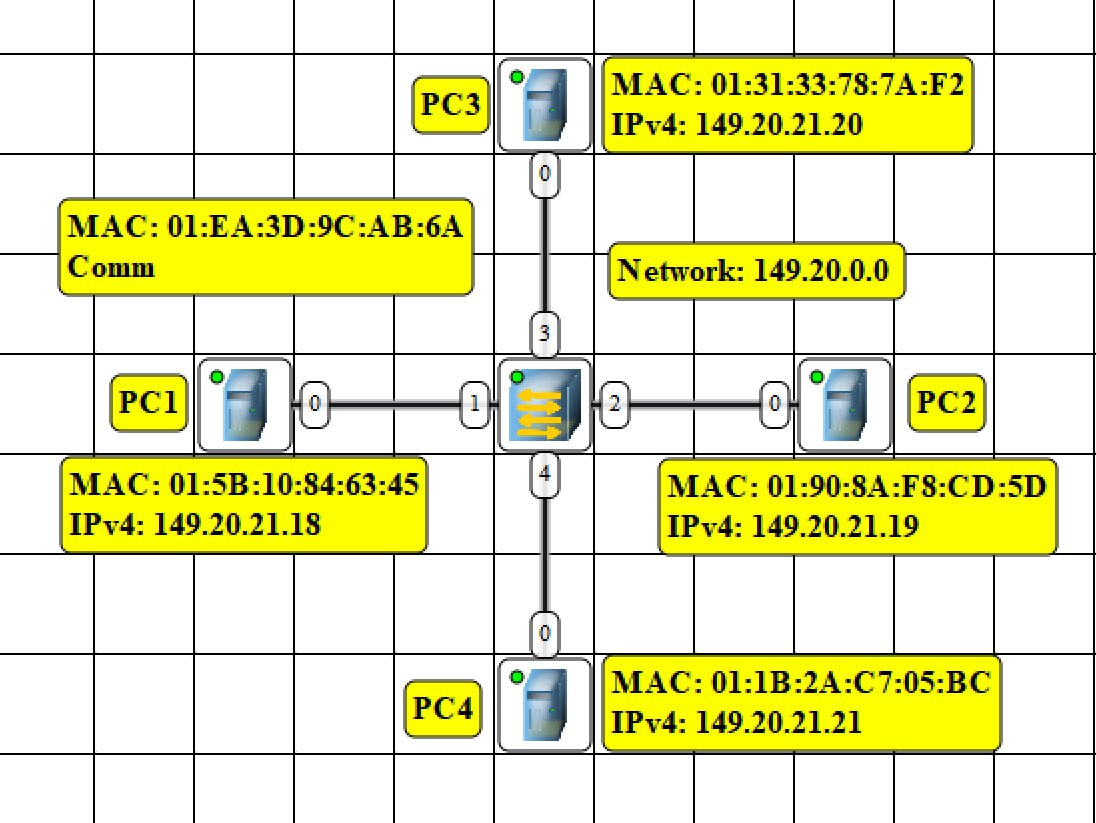
\includegraphics[width=.8\textwidth]{com1.jpg}
\end{center}
Таблица коммутации через некоторое время затишья будет пустая, но я попробовал перед тестированием пересылки описать вручную её LAN порты, чтобы не восстанавливать каждый раз пути.
В отличии от концентратора, который протягивает трафик с одного узла на все остальные, коммутатор передаёт сообщение непосредстенно получателю, если в таблице коммутации внесены определения для устройств.
\begin{center}
    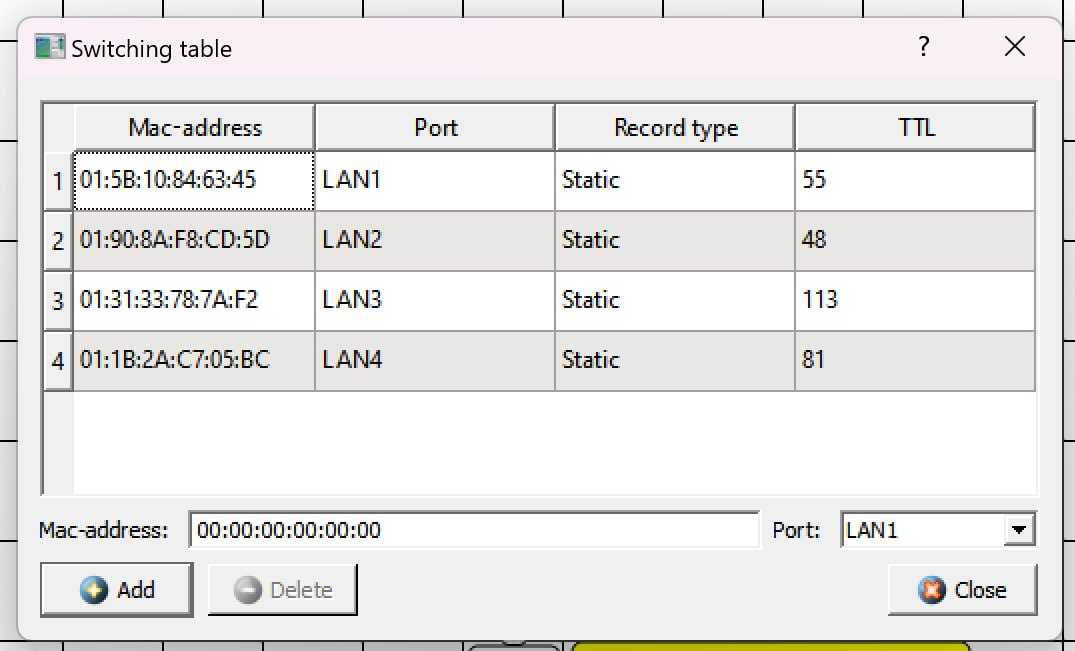
\includegraphics[width=.8\textwidth]{com2.jpg}
\end{center}
Далее были проведены тесты пересылки сообщений по UDP.
\begin{center}
    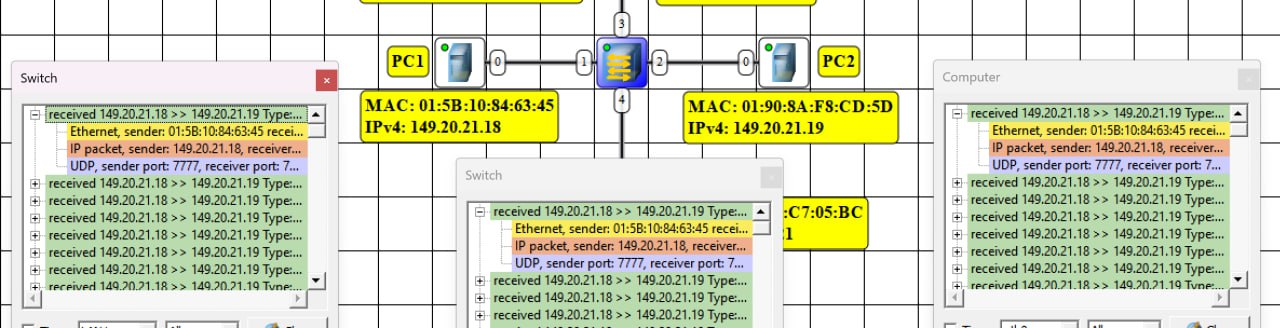
\includegraphics[width=.9\textwidth]{com3.jpg}
\end{center}
И тестирование TCP/IP
(установление соединений)
\begin{center}
    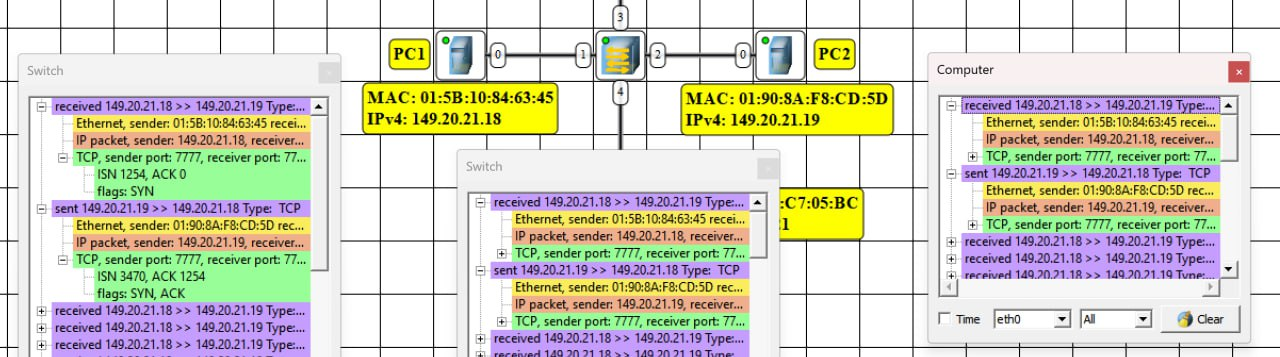
\includegraphics[width=.9\textwidth]{com4.jpg}
\end{center}

(пересылка сообщений)
\begin{center}
    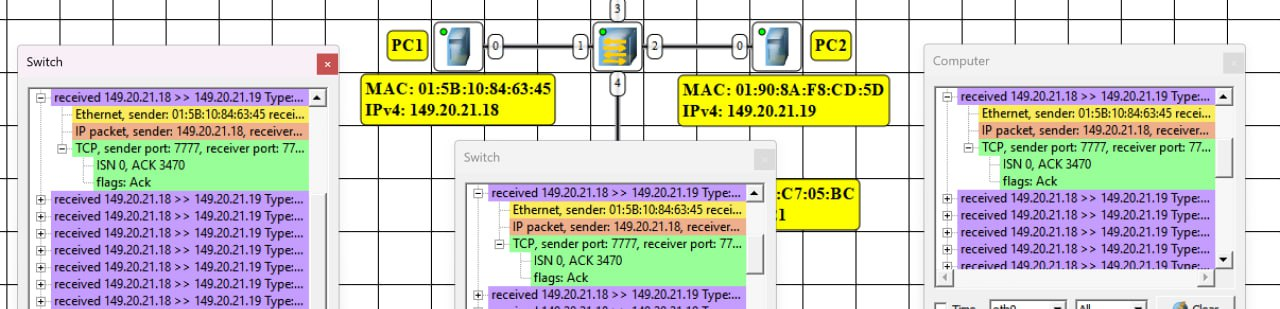
\includegraphics[width=.9\textwidth]{com5.jpg}
\end{center}

\section{Многосегментная локальная сеть}
\begin{center}
    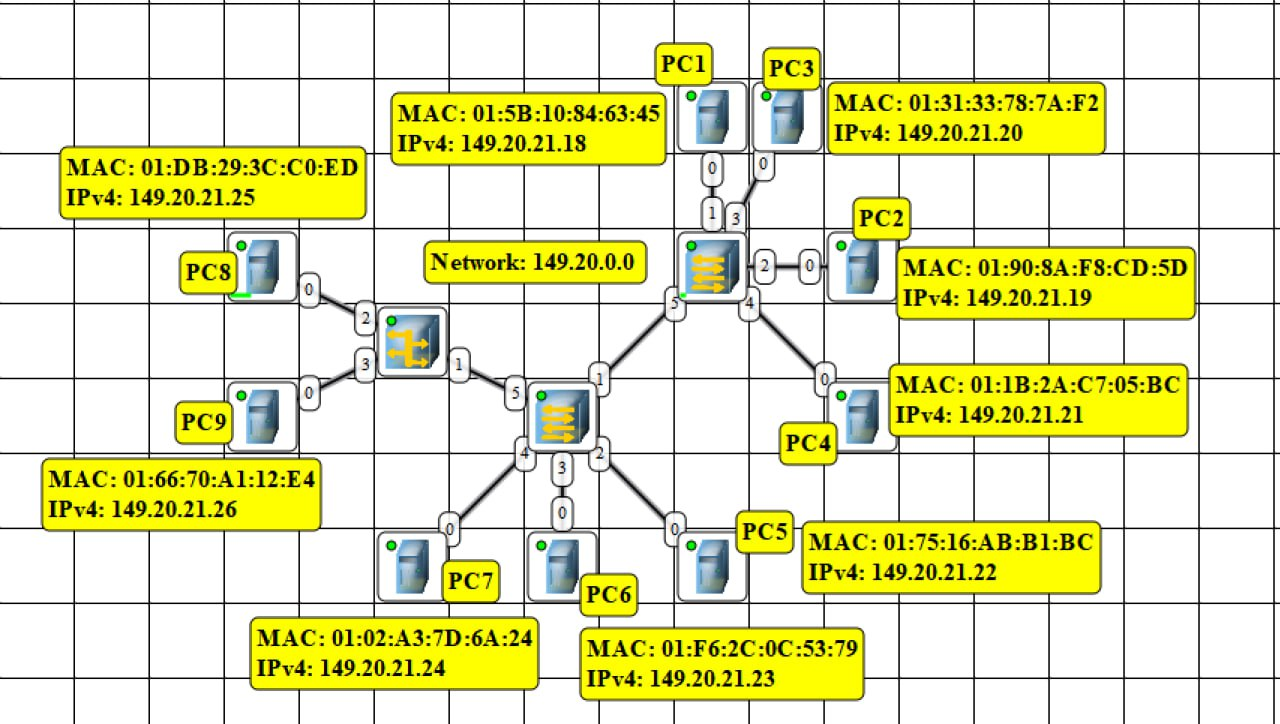
\includegraphics[width=.9\textwidth]{mm1.jpg}
\end{center}
В данном варианте предлагается объединить все предыдующие сети в одну и при этом добавить ещё одну сеть с коммутатором.
Было решено разместить кусок с коммутатором на краю, так как он работает более топорно и если он будет стоять в середине, то каждый раз сообщение будет отправляться во все коммутаторы и излище давать нагрузку. 
Топологии: общая шина. Кольцо сделать не получилось, так как концентратор не может получать и отправлять одновременно более одного сообщения. При замене концентратора на коммутатор, то будет зацикливание сообщения с ответом на зпрос о соединении. 
Так же возможно последовательное подключение вместо шины. 


\section{Вывод}
Изучили принципы настройки и функционирования локальных сетей,
построенных с использованием концентраторов и коммутаторов, а также
процессы передачи данных на основе стека протоколов TCP/IP, с
использованием программы моделирования компьютерных сетей NetEmul.
\end{document}
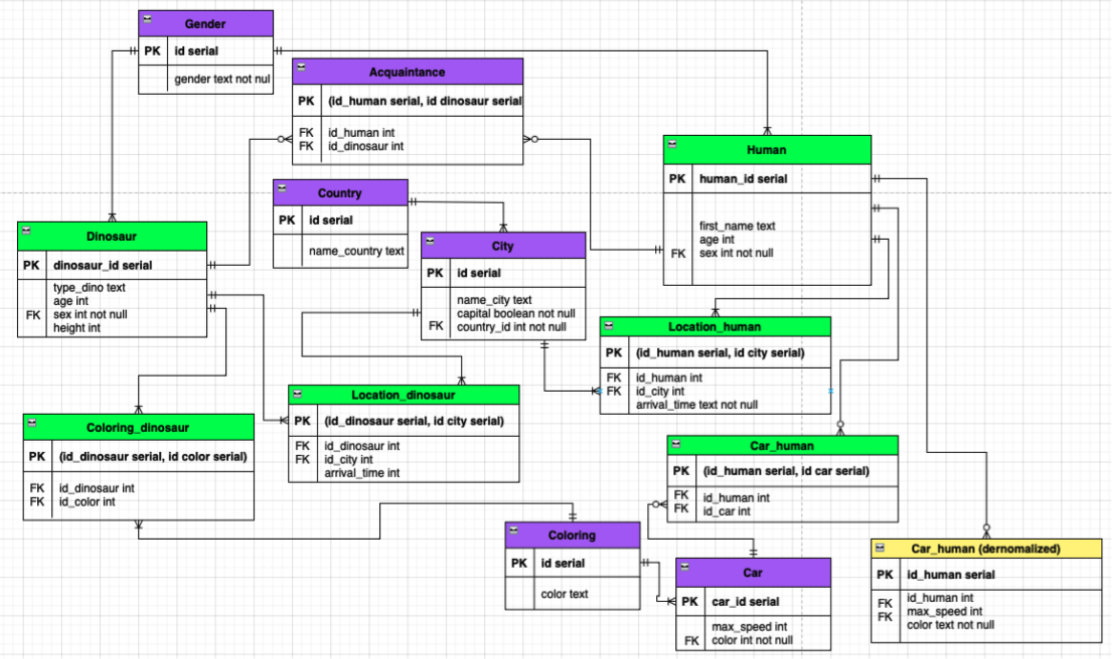
\includegraphics[width=.9\textwidth]{123}